%!TEX root = ../thesis.tex
%*******************************************************************************
%*********************************** Eighth Chapter *****************************
%*******************************************************************************

\chapter{Research of the shape changes of the arterial pulses during proximal occlusions}  %Title of the Chapter
\label{chapter apa}

\ifpdf
\graphicspath{{Chapter7/Figs/Raster/}{Chapter7/Figs/PDF/}{Chapter7/Figs/}}
\else
\graphicspath{{Chapter7/Figs/Vector/}{Chapter7/Figs/}}
\fi

The arterial pulses amplitude (APA) signifies a dynamic component of the impedance plethysmography signal. Importantly, it is located within the basal impedance that accounts for around \SI{0.1}{\percent} of the total waveform \cite{anderson1984impedance}. It can be fairly challenging to acquire these signals since noise levels can be higher than the actual signal, which makes it difficult to isolate this waveform. 

However, such data collection imparts valuable information concerning the haemodynamics per heartbeat. The shape of the waveform has been demonstrated to be a major indicator of haemodynamic problems within the peripheral circulation \cite{ montgomery2011segmental}. This chapter will analyse the waveforms with an aim to differentiate morphological changes between baseline signals and the ones that occur during venous, partial arterial and total occlusion, respectively.

There has been a shift in the impedance baseline occurring during each occlusion. However, it is important to examine the impact that the different kind occlusions of the upper arm within the plethysmography waveforms.  This information offers clues as to whether an occlusion may occur in the arterial or venous circulation.  The iPG device features an output port denominated $Z_{AC}$ that provides a high-resolution view of these arterial pulses waveform.  As illustrated in the design section \ref{section material envelope}, this signal was filtered/amplified as many as almost 2500 times to attain this level of detailing. As a result, the waveform provides more in-depth detail while also improving the signal's noise rejection.

The device was able to deliver an excellent result with regard to filtering and isolation of the APA waveform. However, it goes without saying that some portion of the noise was amplified by the hardware as well. Therefore, further post-processing was necessitated to completely clean up the plethysmography signal. In this regard, tighter filters (see table \ref{table:filters}) were applied in order to remove low and high frequency components. In addition, the lower envelope component was removed and levelled to zero.

The APA waveform produced by this device is inverted, as represented by various other plethysmography methods like photoplethysmography. During the systolic cycle, there is an expansion of blood vessels, which allows for more blood volume. As a result, the impedance declines proportionally to the quantum of blood due to the fact that the forearm's segment is more electrically conductive. Meanwhile during the diastolic cycle, blood vessels end up emptying, causing a decline in the quantity of blood contained within the segment. Consequently, the impedance goes up.

The analysis of plethysmographic wave was carried out by averaging the detected waveforms using specialised algorithms in order to identify an APA signal. The following section discusses the changes within a wave shape from a non-occlusion state to an occluded one. Towards the end of the section, the results of all participants are summarised.

\section{Reference points for the arterial pulse amplitude analysis}
\label{section apa 1}
The isolated APA waveforms reproduce the change in volume per heart beat within the sensing electrodes of the iPG device placed in the forearm. Filling the vessels with blood leads to small changes in resistivity that tend to vary with the circulatory cycle (see section \ref{section procedure flow beat}), describing different peaks during the course of a heart cycle.

\begin{figure}[!htpb]
	\centering
	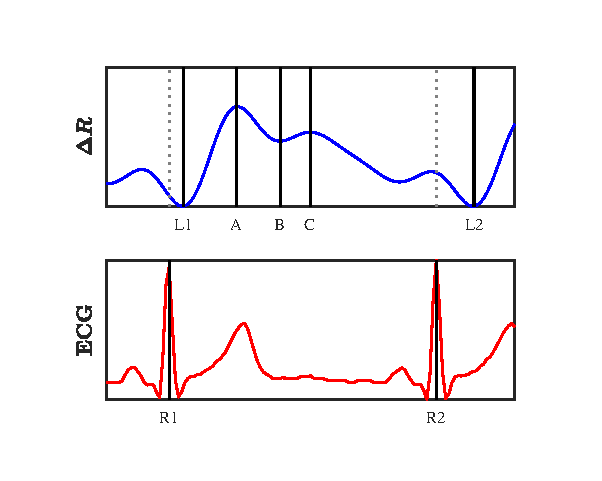
\includegraphics[width=10cm,keepaspectratio]{figure_apa_1}
	\caption[Marker ppoints in an iPG waveform]{Peaks and valleys of an iPG waveform ($\Delta R$) compared to ECG waveform.}
	\label{fig:markers iPG}
\end{figure}

Commonly, an APA wave consists of several identifiable peaks and valleys. Figure \ref{fig:markers iPG} illustrates a typical impedance plethysmography pulse synchronous with a heartbeat in addition to a limb. The table \ref{tbl:APA markers} summarises the noticeable markers of these pulse waveforms when compared to an ECG.

\begin{table}[!htpb]
	\caption{Markers on the APA waveform}
	\label{tbl:APA markers}
	\centering
	\begin{tabular}{c p{10cm}}
		\textbf{Marker} & \textbf{Description} \\
		\toprule
		R1 & Peak of the ECG QRS complex before an APA pulse. \\
		L1 & Start of the systolic upslope of the APA signal. Point where  rapid change of impedance occurs. \\
		A & Systolic point. Maximum peak of the APA signal.  \\
		B & Dicrotic notch on the APA wave. \\
		C & Maximum pulse after the dicrotic notch, named diastolic pulse  \\
		R2 & Peak of the ECG QRS complex after the APA pulse.  \\
		L2 & Starting point of the next APA wave. \\
		\bottomrule
	\end{tabular}
\end{table}

An APA wave needs to be identified as a valid one in order to be included in the computational analysis. As a result, the programmed algorithm begins with the identification of the commencement and end of a pulse by locating the upslope point $L1$ as well as $L2$ in the waveform. Upon the identification of this spot, the systolic peak $A$ can be placed. The point $B$ is expected to be a valley with an amplitude lower than the previous peak. Subsequently, the algorithm looks at the following change of slope - the diastolic peak $C$. If any of these conditions could not be met, the algorithm searches through the APA wave from the subsequent lower data point, seeking a matching wave pattern again. In case a pattern is found ($L1 > A < B > slope change (C) > L2$), this is considered as a fixed wave. In the absence of a match, the pulse is marked as missing. In order to minimise waves with abnormal amplitudes caused due to noise, the algorithm then calculates the mean peak at $A$ of the last 20 valid APA waves. If this value is found to be greater than \SI{25}{\percent} ($A > A*1.25$) the wave is discarded.

The table \ref{tbl:detect APA} compiles the amount of APA waves recognised by the algorithm. The column \textit{detected waves} describes the pulses that adhere to the profile of an iPG plethysmography wave. Meanwhile the third column highlights the pulses that did not match the anticipated guide; subsequently, the algorithm attempted to fix them by identifying the pattern within the next slope. Consequently, the fixed column shows the total amount of identified pulse, whereas the last column shows the one that are discarded.

Generally speaking, the quality of APA pulses validated by the iPG device and verified by the algorithm were on average \SI{57.86(1637)}{\percent}. Participants 3, 4 and 8 showed the highest number of pulses with errors (above \SI{50}{\percent}). However, by incorporating the fixing method, the number of valid peaks improved to a total of \SI{84.94(764)}{\percent}.

\begin{table}[!htbp]
	\caption[Total amount of iPG waves detected by the algorithm]{Total amount of iPG waves detected by the algorithm. Starting form the detection of valleys follow by the detection of systolic peak, dicrotic notch point and diastolic peak. It also includes the waves reconstructed by the software}
	\label{tbl:detect APA}
	\centering\small
	\begin{tabular}{lrrr>{\columncolor[gray]{0.8}}l>{\columncolor[gray]{0.9}}l}
		\toprule
		& \multicolumn{1}{c}{\textbf{Total}}
		& \multicolumn{1}{c}{\textbf{Detected}} & \multicolumn{1}{c}{\textbf{Waves}}& \multicolumn{1}{c}{\textbf{Fixed}} & \multicolumn{1}{c}{\textbf{Discarded}} \\
		& \multicolumn{1}{c}{\textbf{valleys}} & \multicolumn{1}{c}{\textbf{waves}} & \multicolumn{1}{c}{\textbf{with errors}}& \multicolumn{1}{c}{\textbf{waves}} & \multicolumn{1}{c}{\textbf{waves}} \\
		\midrule
		Participant 1	&1604	& 840 (\SI{52.37}{\percent})	&764 (\SI{47.63}{\percent})	&491 (\SI{30.61}{\percent})	&273 (\SI{17.02}{\percent})\\
		Participant 2	&1689	&1159 (\SI{68.62}{\percent})	&530 (\SI{31.38}{\percent})	&409 (\SI{24.22}{\percent})	&121 ( \SI{7.16}{\percent})\\
		Participant 3	&1651	& 699 (\SI{42.34}{\percent})	&952 (\SI{57.66}{\percent})	&695 (\SI{42.10}{\percent})	&257 (\SI{15.57}{\percent})\\
		Participant 4	&1625	& 645 (\SI{39.69}{\percent})	&980 (\SI{60.31}{\percent})	&562 (\SI{34.58}{\percent})	&418 (\SI{25.72}{\percent})\\
		Participant 5	&1664	&1199 (\SI{72.06}{\percent})	&465 (\SI{27.94}{\percent})	&345 (\SI{20.73}{\percent})	&120 ( \SI{7.21}{\percent})\\
		Participant 6	&1745	& 936 (\SI{53.64}{\percent})	&809 (\SI{46.36}{\percent})	&471 (\SI{26.99}{\percent})	&338 (\SI{19.37}{\percent})\\
		Participant 7	&1907	&1654 (\SI{86.73}{\percent})	&253 (\SI{13.27}{\percent})	&146 ( \SI{7.66}{\percent})	&107 ( \SI{5.61}{\percent})\\
		Participant 8	&1651	& 784 (\SI{47.49}{\percent})	&867 (\SI{52.51}{\percent})	&491 (\SI{29.74}{\percent})	&376 (\SI{22.77}{\percent})\\
		\bottomrule
	\end{tabular}
\end{table}

On the basis of data, the changes that took place during each occlusion among the points $A$, $B$ and $C$ were examined. The following analysis centres on the changes of impedance amplitude all along the different regions of this experiment, as well as the change of area of the waveform before and after the dicrotic notch point ($B$).

\section{Changes of the plethysmography waveform during different occlusions}
\label{section apa 2}
The detection of the APA waveforms makes it possible to independently analyse the change of the shape form. To that end, an average waveform was computed for all these regions during the experiment. The following section details the relevant changes made for each of these points of interest. 

\subsection{Plethysmography waveform change during venous occlusion}
\label{section apa 2.1}
The analysis performed in this section corresponds to the APA waveforms captured during the baseline in region 1 (\SIrange{0}{300}{\second}), venous occlusion (\SIrange{300}{480}{\second}) and return to control signal (\SIrange{480}{780}{\second}).  The previous section described the method of collecting valid pulses. Consequently, all other valid pulses were grouped and aligned as per region to calculate the average waveform. 

Figure \ref{fig:iPG_venous_baseline} shows an impedance plethysmography waveform that was calculated by one of the participants during baseline and venous occlusion, with indicators of their amplitudes located at different points of interest. Some of these markers show the calculation of distance between systolic peak (Point A) to dicrotic notch (Point B) and diastolic peak (Point C), along with the amplitude for each of these markers. The distance between (A $\rightarrow$ B) and (A $\rightarrow$ C) was later transposed into the occlusion wave in order to identify their values during the VOP test. Clearly, from a qualitative viewpoint, a difference can be noticed in the morphology of the waveform that occurred during the occlusion.  Indeed, figure \ref{fig:iPG change points venous} shows the change in amplitude at these points for every participant as well as the return to baseline after releasing the cuff pressure. A comprehensive analysis of this change (at each point) is detailed in the following manner.

%This method allows multifigures being aligned using subcaptionbox
\begin{figure*}[!htbp]
	\centering
	\null\hfill%
	\subcaptionbox{Average APA waveform for baseline region 1 (\SIrange{0}{300}{\second})\label{fig:iPG_venous_baseline}}
	[0.48\textwidth]{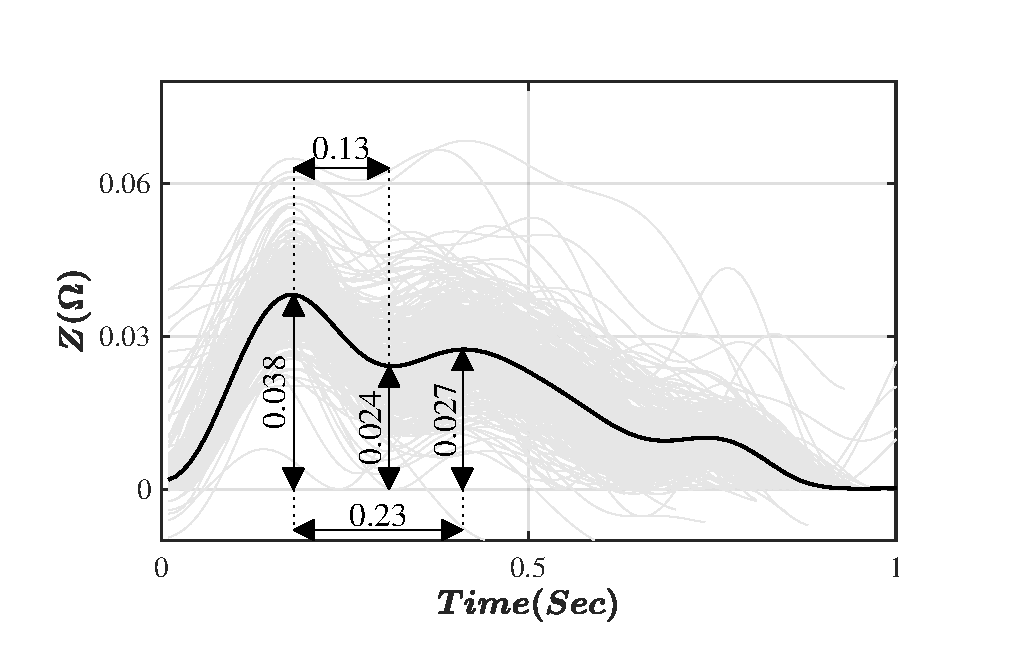
\includegraphics[width=0.48\textwidth, trim={0.5cm 0cm 1.5cm 0 cm}, clip]{figure_apa_2a}}%
	\hfill%
	\subcaptionbox{Average APA waveform during venous occlusion region 2 (\SIrange{300}{480}{\second})\label{fig:iPG_venous_occlusion}}
	[0.48\textwidth]{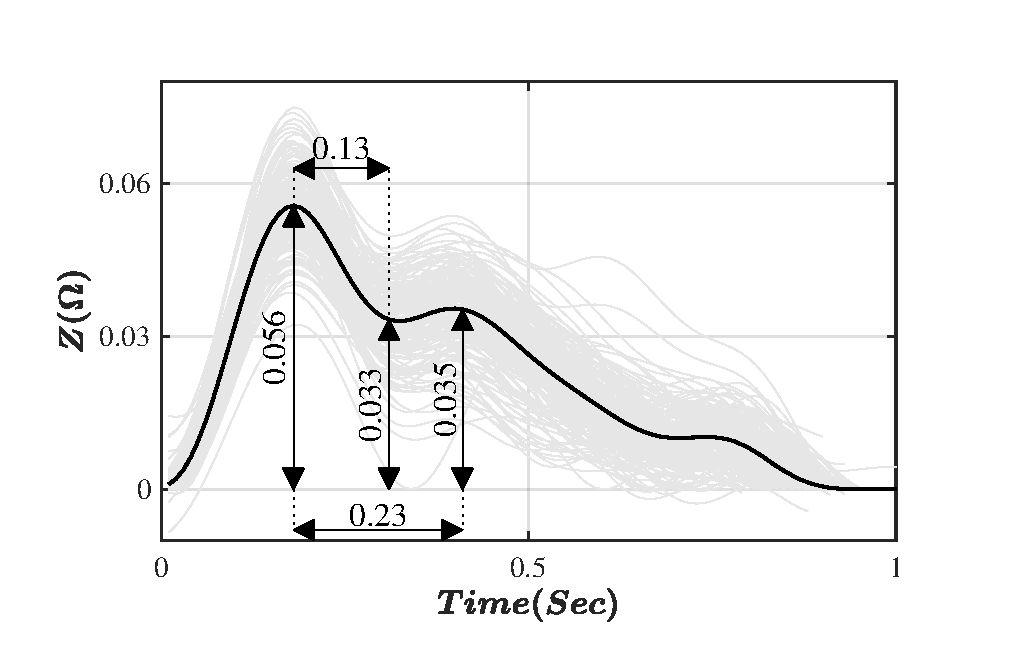
\includegraphics[width=0.48\textwidth, trim={0.5cm 0cm 1.5cm 0 cm}, clip]{figure_apa_2b}}%
	\hfill\null%
	\caption{Plethysmography waveform of the participant seven between baseline and venous occlusion}
	\label{fig:iPG_venous}
	
	\vspace{1cm}
	
	\null\hfill%
	\subcaptionbox{Change of amplitude of the waveform at point A.\label{fig:change A venous}}
	[0.48\textwidth]{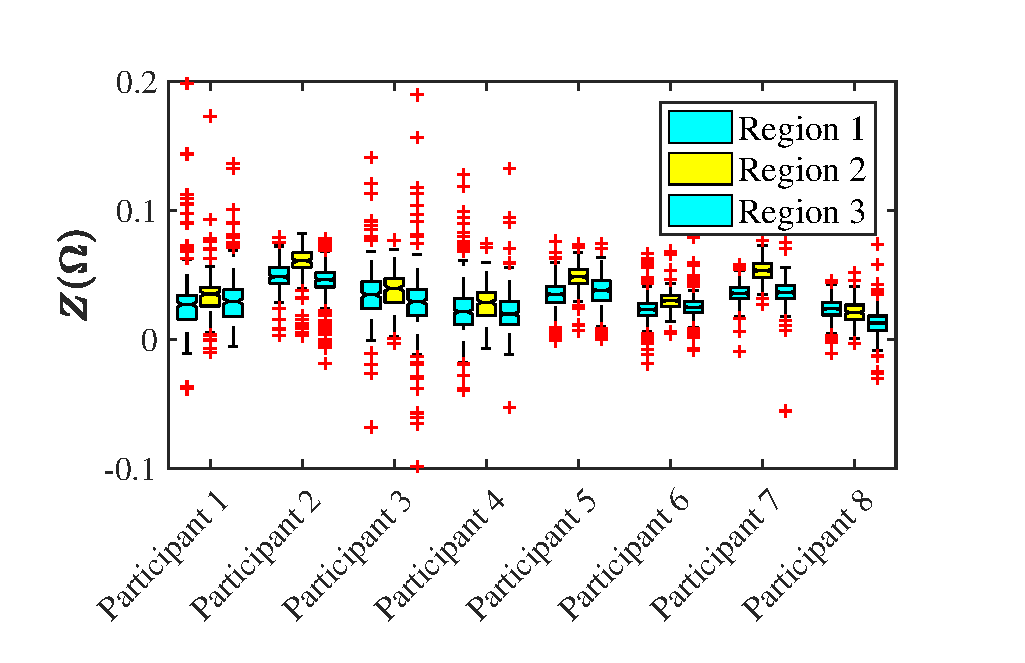
\includegraphics[width=0.45\textwidth, trim={0.5cm 0cm 1.5cm 0 cm}, clip]{figure_apa_3a}}%
	\hfill%
	\subcaptionbox{Change of amplitude of the waveform at point B.\label{fig:change B venous}}
	[0.48\textwidth]{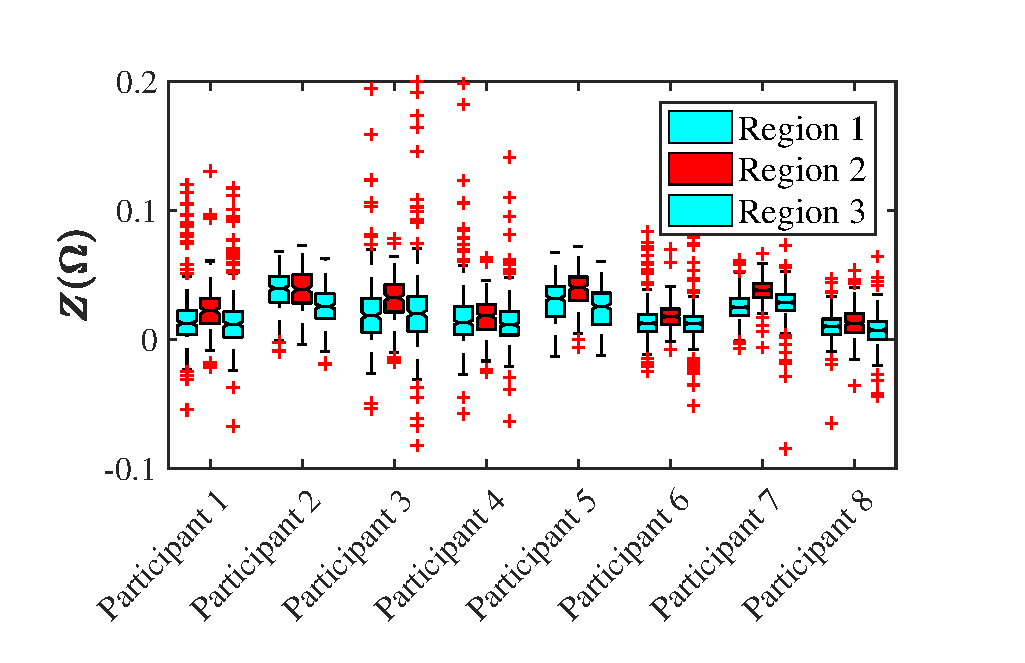
\includegraphics[width=0.45\textwidth, trim={0.5cm 0cm 1.5cm 0 cm}, clip]{figure_apa_3b}}%
	\hfill%
	\subcaptionbox{Change of amplitude of the waveform at point C.\label{fig:change C venous}}
	[0.48\textwidth]{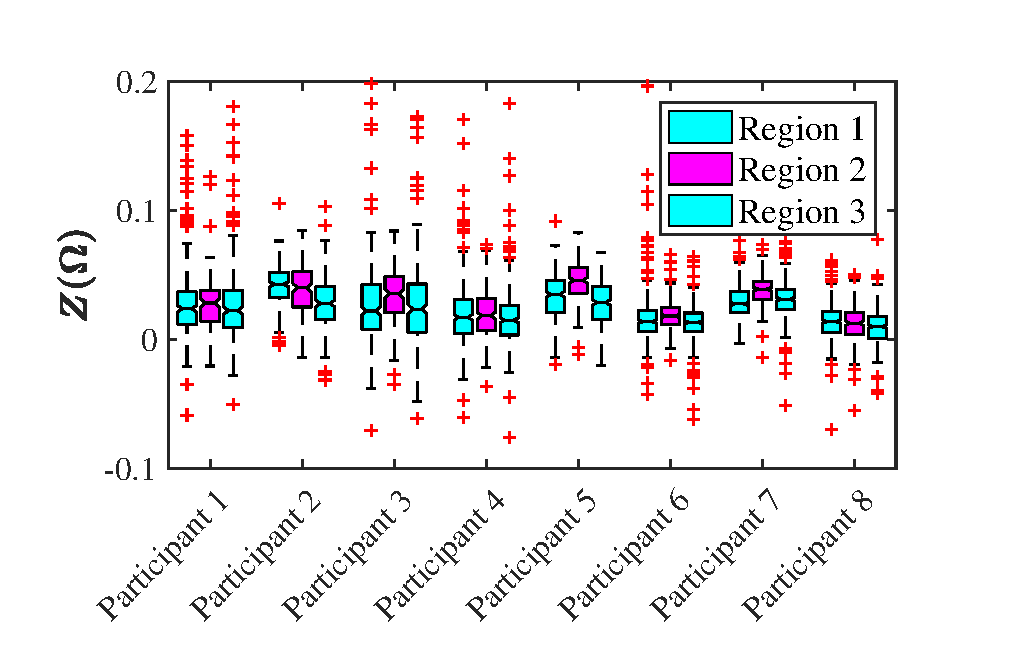
\includegraphics[width=0.45\textwidth, trim={0.5cm 0cm 1.5cm 0 cm}, clip]{figure_apa_3c}}%
	\null%
	\caption{Changes of the impedance peak values during baseline, venous occlusion and return to baseline for points A,B and C.}
	\label{fig:iPG change points venous}
\end{figure*}


\subsubsection{Changes in systolic peak (Point A)}
\label{section apa 2.1.1}
Figure \ref{fig:change A venous} shows the statistical variation of the systolic peak magnitude (point A) during the three conditions of the test baseline-occlusion-baseline. After the cuff was inflated below the diastolic pressure, most APA signals showed an increase of the impedance magnitude of this peak. As detailed in table \ref{tbl:change A venous}, \SI{87}{\percent} of the participants exhibited an increment in electrical resistance during the venous occlusion of about \SI{31.80}{\percent}; the lone exception was participant 8 where his/her impedance dropped in \SI{-12.01}{\percent}. When the cuff's pressure got released, all participants showed a decline in peak value with an average of \SI{-32.21}{\percent}, returning to similar baseline values prior to the venous occlusion.

\begin{table}[!htbp]
	\caption[Change of amplitude of the waveform at peak A during the transition baseline-venous occlusion-baseline.]{Change of amplitude of the waveform at peak \textit{A} during the transition from baseline (region 1), venous occlusion (region 2) and the return to baseline (region 3). The column change shows the percentile variations between the different regions.}
	\label{tbl:change A venous}
	\centering\small
	\begin{tabular}{l
			*{3}{S[table-format=1.4]@{\,\( \pm \)\,}S[table-format=1.4]} %Format for Z+-std
			>{\columncolor[gray]{0.8}}c>{\columncolor[gray]{0.9}}c}
		\toprule
		\multirow{2}{*}{\textbf{Peak A}}
		& \multicolumn{2}{c}{\textbf{Baseline [\si{\ohm}]}}
		& \multicolumn{2}{c}{\textbf{Occlusion [\si{\ohm}]}}
		& \multicolumn{2}{c}{\textbf{Baseline [\si{\ohm}]}}
		& \multicolumn{2}{c}{\textbf{Change}} \\
		& \multicolumn{2}{c}{\colorbox{mycyan}{(Region 1)}}
		& \multicolumn{2}{c}{\colorbox{yellow}{(Region 2 - VO)}}
		& \multicolumn{2}{c}{\colorbox{mycyan}{(Region 3)}}
		&\textbf{R1-R2}&\textbf{R2-R3}\\\midrule
		Participant 1 & 0.0270 & 0.0233 & 0.0353 & 0.0191 & 0.0295 & 0.0305 & 30.49 \% & -21.41 \% \\
		Participant 2 & 0.0485 & 0.0102 & 0.0609 & 0.0140 & 0.0462 & 0.0449 & 25.50 \% & -30.24 \% \\
		Participant 3 & 0.0345 & 0.0351 & 0.0397 & 0.0144 & 0.0292 & 0.0294 & 14.96 \% & -30.55 \% \\
		Participant 4 & 0.0214 & 0.0303 & 0.0289 & 0.0139 & 0.0197 & 0.0222 & 35.17 \% & -43.11 \% \\
		Participant 5 & 0.0352 & 0.0112 & 0.0485 & 0.0098 & 0.0382 & 0.0376 & 37.99 \% & -29.20 \% \\
		Participant 6 & 0.0232 & 0.0105 & 0.0300 & 0.0124 & 0.0249 & 0.0251 & 29.16 \% & -21.77 \% \\
		Participant 7 & 0.0357 & 0.0080 & 0.0534 & 0.0081 & 0.0365 & 0.0365 & 49.33 \% & -47.17 \% \\
		Participant 8 & 0.0238 & 0.0094 & 0.0209 & 0.0091 & 0.0128 & 0.0127 &-12.01 \% & -34.27 \% \\ \bottomrule
	\end{tabular}
\end{table}


\subsubsection{Changes in dicrotic notch peak (Point B)}
\label{section apa 2.1.2}
It can be seen that dicrotic notch (point B) is situated between the systolic (point A) and diastolic peaks (point C), as illustrated in figure \ref{fig:markers iPG}.  Similarly, in congruity with the changes experienced by the systolic peak during this part of the experiment, point B also ended up increasing in its magnitude. Subsequently, when the cuff's pressure got released, the amplitude at this location returned to a level that was fairly close to the baseline. 

Based on the data shown in Table \ref{tbl:change B venous}, it can be noticed that most of the participants (\SI{87.5}{\percent}) exhibited an increase in magnitude of their dicrotic notch point. Among those who experienced this increment, the impedance was seen to change roughly \SI{47.73}{\percent} as compared to the measurement seen at region 1. However, partaker two observed a slight decrease in her measured impedance \SI{-2.06}{\percent} which did not assume much significance when compared to others. In contrast, after releasing the upper arms blockage, all participants experienced a decline in their point B magnitude of about  \SI{-51.68}{\percent}.

\begin{table}[!htbp]
	\caption[Change of amplitude of the waveform at peak B during the transition baseline-venous occlusion-baseline.]{Change of amplitude of the waveform at peak \textit{B} during the transition from baseline (region 1), venous occlusion (region 2) and the return to baseline (region 3). The column change shows the percentile variations between the different regions.}
	\label{tbl:change B venous}
	\centering\small
	\begin{tabular}{l
			*{3}{S[table-format=1.4]@{\,\( \pm \)\,}S[table-format=1.4]} %Format for Z+-std
			>{\columncolor[gray]{0.8}}c>{\columncolor[gray]{0.9}}c}
		\toprule
		\multirow{2}{*}{\textbf{Peak B}}
		& \multicolumn{2}{c}{\textbf{Baseline [\si{\ohm}]}}
		& \multicolumn{2}{c}{\textbf{Occlusion [\si{\ohm}]}}
		& \multicolumn{2}{c}{\textbf{Baseline [\si{\ohm}]}}
		& \multicolumn{2}{c}{\textbf{Change}} \\
		& \multicolumn{2}{c}{\colorbox{mycyan}{(Region 1)}}
		& \multicolumn{2}{c}{\colorbox{myred}{(Region 2 - VO)}}
		& \multicolumn{2}{c}{\colorbox{mycyan}{(Region 3)}}
		&\textbf{R1-R2}&\textbf{R2-R3}\\\midrule
		Participant 1 & 0.0126 & 0.0231 & 0.0223 & 0.0195 & 0.0119 & 0.0153 & 76.94 \% & -82.52 \% \\
		Participant 2 & 0.0397 & 0.0144 & 0.0388 & 0.0167 & 0.0257 & 0.0252 & -2.06 \% & -33.19 \% \\
		Participant 3 & 0.0184 & 0.0315 & 0.0323 & 0.0181 & 0.0200 & 0.0224 & 75.98 \% & -67.36 \% \\
		Participant 4 & 0.0130 & 0.0294 & 0.0183 & 0.0149 & 0.0113 & 0.0138 & 40.21 \% & -53.52 \% \\
		Participant 5 & 0.0319 & 0.0158 & 0.0402 & 0.0138 & 0.0254 & 0.0237 & 25.92 \% & -46.26 \% \\
		Participant 6 & 0.0127 & 0.0138 & 0.0177 & 0.0161 & 0.0124 & 0.0128 & 39.75 \% & -41.55 \% \\
		Participant 7 & 0.0250 & 0.0108 & 0.0382 & 0.0092 & 0.0287 & 0.0276 & 52.71 \% & -37.97 \% \\
		Participant 8 & 0.0102 & 0.0111 & 0.0125 & 0.0117 & 0.0073 & 0.0071 & 22.58 \% & -51.08 \% \\
		\bottomrule
	\end{tabular}
\end{table}

\subsubsection{Changes in diastolic peak (Point C)}
\label{section apa 2.1.3}
The last analysed peak corresponds to point C or the diastolic peak of the waveform. To reiterate, figure \ref{fig:change C venous} illustrates that most of these participants (\SI{71.4}{\percent}) exhibited an increase in magnitude of about \SI{31.92}{\percent} as compared to region 1. Only participants 2 and 8 witnessed a slight decline in their impedance on an average of \SI{-7.97}{\percent}. 

Table \ref{tbl:change C venous} illustrates the mean values of impedance at this location within the waveform. In contrast, after releasing the pressure from the upper arm, a decrease was observed in the diastolic peak impedance of all participants, at an average of \SI{-32.33}{\percent}. As a result, the diastolic peak returned to values that were similar to the baseline, barring the ones that experienced a diminished resistance during the occlusion.

\begin{table}[!htbp]
	\caption[Change of amplitude of the waveform at peak C during the transition baseline-venous occlusion-baseline.]{Change of amplitude of the waveform at peak \textit{C} during the transition from baseline (region 1), venous occlusion (region 2) and the return to baseline (region 3). The column change shows the percentile variations between the different regions.}
	\label{tbl:change C venous}
	\centering\small
	\begin{tabular}{l
			*{3}{S[table-format=1.4]@{\,\( \pm \)\,}S[table-format=1.4]} %Format for Z+-std
			>{\columncolor[gray]{0.8}}c>{\columncolor[gray]{0.9}}c}
		\toprule
		\multirow{2}{*}{\textbf{Peak C}}
		& \multicolumn{2}{c}{\textbf{Baseline [\si{\ohm}]}}
		& \multicolumn{2}{c}{\textbf{Occlusion [\si{\ohm}]}}
		& \multicolumn{2}{c}{\textbf{Baseline [\si{\ohm}]}}
		& \multicolumn{2}{c}{\textbf{Change}} \\
		& \multicolumn{2}{c}{\colorbox{mycyan}{(Region 1)}}
		& \multicolumn{2}{c}{\colorbox{mymagenta}{(Region 2 - VO)}}
		& \multicolumn{2}{c}{\colorbox{mycyan}{(Region 3)}}
		&\textbf{R1-R2}&\textbf{R2-R3}\\\midrule
		Participant 1 & 0.0238 & 0.0281 & 0.0283 & 0.0260 & 0.0224 & 0.0286 & 18.81 \% & -24.75 \% \\
		Participant 2 & 0.0429 & 0.0150 & 0.0401 & 0.0191 & 0.0279 & 0.0278 & -6.48 \% & -28.45 \% \\
		Participant 3 & 0.0221 & 0.0397 & 0.0355 & 0.0219 & 0.0236 & 0.0310 & 60.85 \% & -53.94 \% \\
		Participant 4 & 0.0171 & 0.0380 & 0.0184 & 0.0174 & 0.0149 & 0.0178 &  7.42 \% & -20.30 \% \\
		Participant 5 & 0.0350 & 0.0175 & 0.0459 & 0.0151 & 0.0287 & 0.0279 & 31.16 \% & -49.18 \% \\
		Participant 6 & 0.0138 & 0.0212 & 0.0182 & 0.0251 & 0.0133 & 0.0151 & 31.53 \% & -35.22 \% \\
		Participant 7 & 0.0276 & 0.0127 & 0.0391 & 0.0111 & 0.0312 & 0.0309 & 41.77 \% & -28.58 \% \\
		Participant 8 & 0.0138 & 0.0140 & 0.0125 & 0.0163 & 0.0100 & 0.0096 & -9.47 \% & -18.24 \% \\
		
		\bottomrule
	\end{tabular}
\end{table}

\subsection{Plethysmography waveform shift during partial arterial occlusion}
\label{section apa 2.2}
During the partial occlusion of the brachial artery, majority of the participants exhibited a change in shape of their waveforms. An analysis of this section resembles the baseline time outlined in region 3 (\SIrange{480}{780}{\second}), three minutes of the partial venous occlusion in region 4 (\SIrange{780}{960}{\second}) and a return to baseline region 5 (\SIrange{960}{1260}{\second}).  Next, the cuff was inflated to the pressure presented in column \textit{Occlusion 2} in Table \ref{tbl: venous occlusions}, laying between diastolic and systolic pressures.

Figure \ref{fig:iPG arterial} illustrates the average waveform of all signals that were aligned at baseline and during the arm's occlusion for one of these participants. Evidently, there is a surge in the systolic peak (point A), and  a reduction in the diastolic peak at point C. Figure \ref{fig:iPG change points arterial} also highlights the impedance change in all participants during the three regions. The following sections will describe the changes made in each of the spots in greater detail.

%This method allows multifigures being aligned using subcaptionbox
\begin{figure*}
	\centering
	\null\hfill%
	\subcaptionbox{Average baseline plethysmography waveform before partial arterial occlusion region 3 (\SIrange{480}{780}{\second})\label{fig:iPG arterial baseline}}
	[0.45\textwidth]{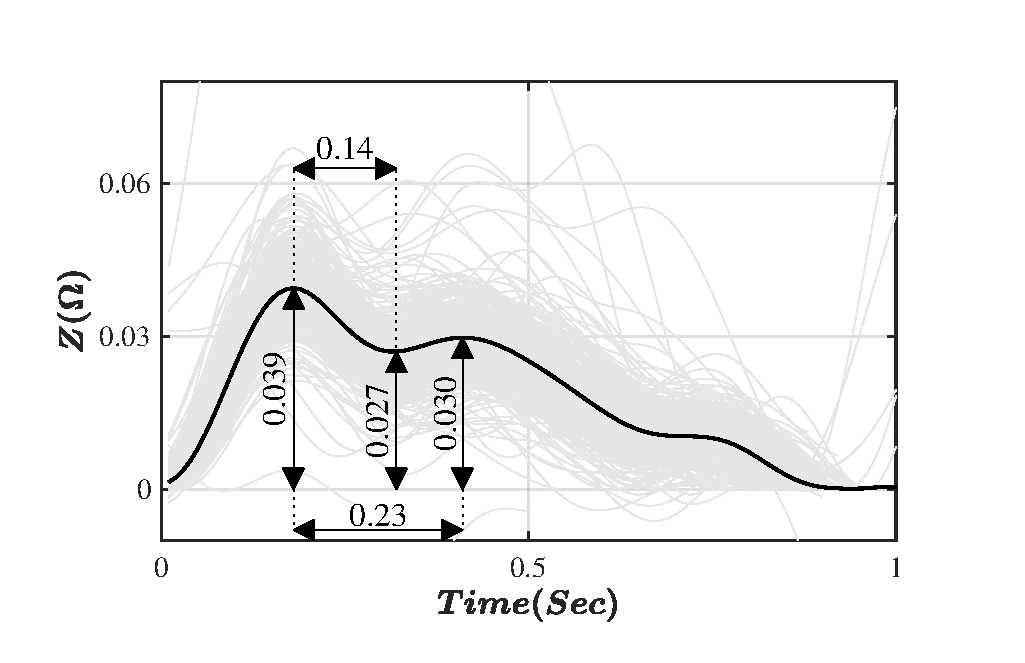
\includegraphics[width=0.45\textwidth, trim={0.5cm 0cm 1.5cm 0 cm}, clip]{figure_apa_4a}}%
	\hfill%
	\subcaptionbox{Average plethysmography waveform during partial arterial occlusion region 4 (\SIrange{780}{960}{\second})\label{fig:iPG arterial occlusion}}
	[0.45\textwidth]{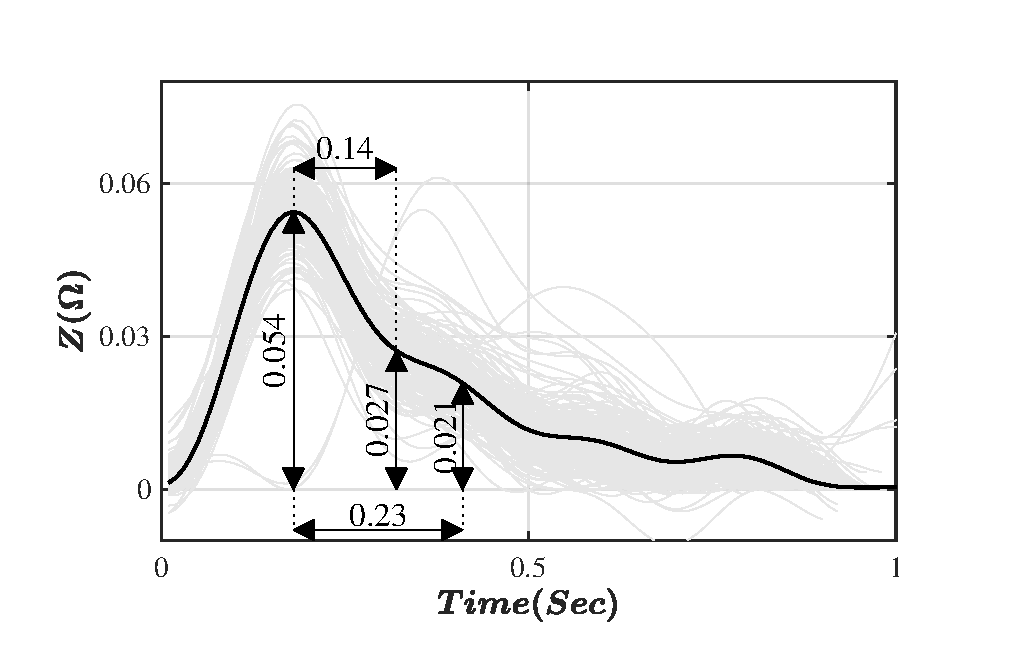
\includegraphics[width=0.45\textwidth, trim={0.5cm 0cm 1.5cm 0 cm}, clip]{figure_apa_4b}}%
	\hfill\null%
	\caption{Plethysmography waveform of the participant seven between baseline and partial arterial occlusion}
	\label{fig:iPG arterial}
	
	\vspace{1cm}
	
	\null\hfill%
	\subcaptionbox{Change of amplitude of the waveform at point A.\label{fig:change A arterial}}
	[0.48\textwidth]{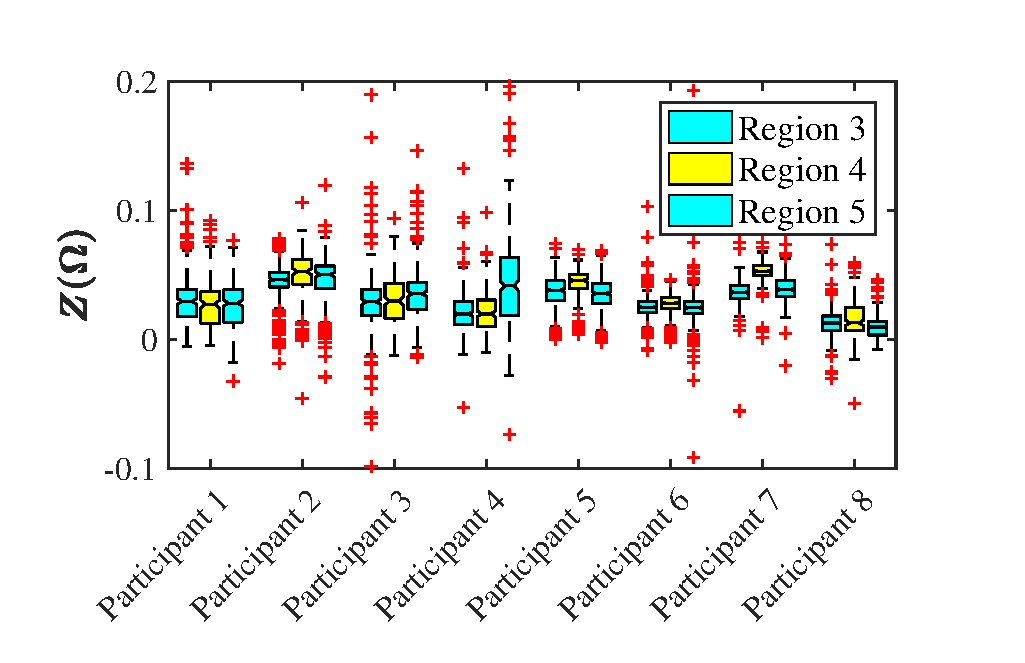
\includegraphics[width=0.45\textwidth, trim={0.5cm 0cm 1.5cm 0 cm}, clip]{figure_apa_5a}}%
	\hfill%
	\subcaptionbox{Change of amplitude of the waveform at point B.\label{fig:change B arterial}}
	[0.48\textwidth]{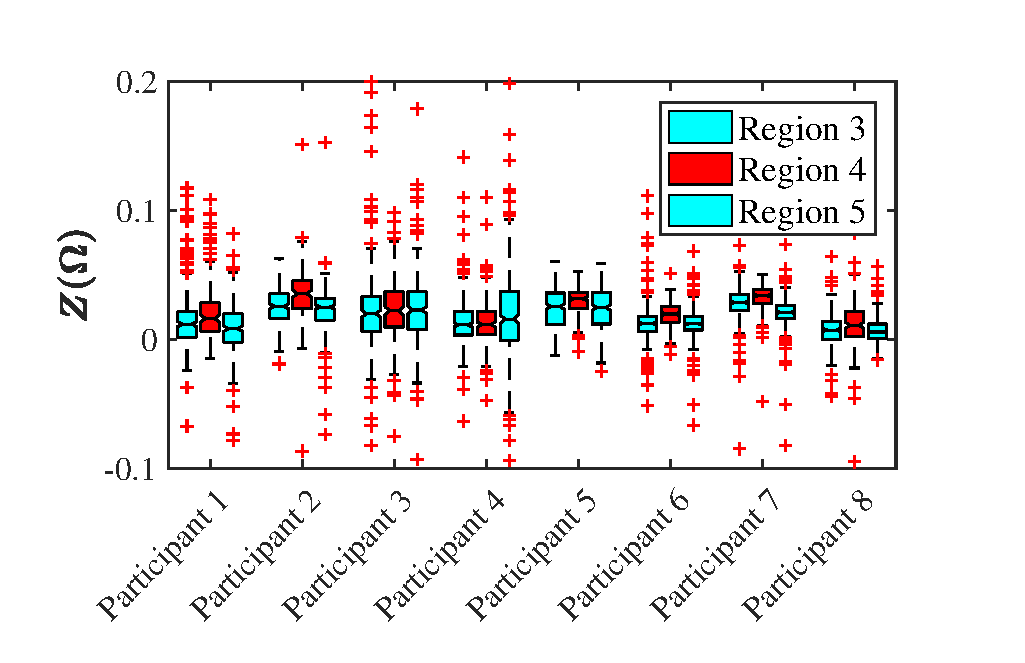
\includegraphics[width=0.45\textwidth, trim={0.5cm 0cm 1.5cm 0 cm}, clip]{figure_apa_5b}}%
	\hfill%
	\subcaptionbox{Change of amplitude of the waveform at point C.\label{fig:change C arterial}}
	[0.48\textwidth]{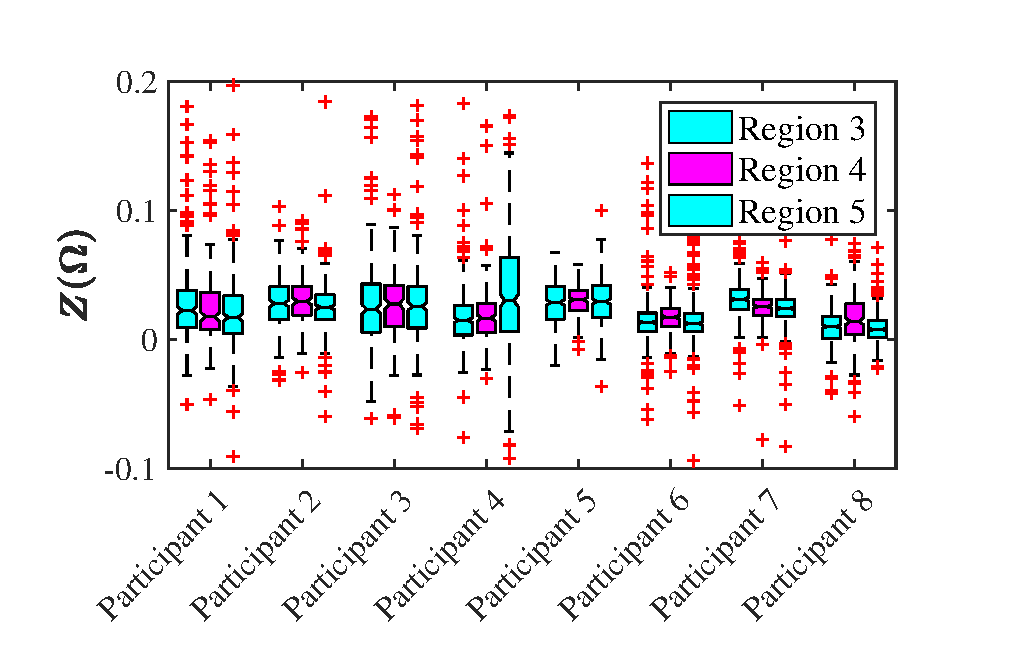
\includegraphics[width=0.45\textwidth, trim={0.5cm 0cm 1.5cm 0 cm}, clip]{figure_apa_5c}}%
	\null%
	\caption{Changes of the impedance peak values during baseline, partial arterial occlusion and return to baseline for points A,B and C.}
	\label{fig:iPG change points arterial}
\end{figure*}

\subsubsection{Changes in systolic peak (Point A)}
\label{section apa 2.2.1}
Figure \ref{fig:change A arterial} illustrates the change in amplitude for each participant. In addition, table \ref{tbl:change A arterial} summarises the average impedances along with the variations in each region. Through this occlusive experiment, seven participants (\SI{87.5}{\percent}) showed an increase in electrical resistivity at point A of about \SI{13.52}{\percent}. However, some of them exhibited a small surge in their peaks between \SIrange{0.29}{2.24}{\percent}. In general, the increase at this point can be observed. After the deflation of the cuff, most participants (\SI{62.5}{\percent}) exhibited a decline in peak on an average of \SI{-21.86}{\percent}.  In contrast, participants 1, 3 and 4 registered an increase in impedance reading, the latter being an outlier with a hike in his magnitude of \SI{110.69}{\percent}.

\begin{table}[!htbp]
	\caption[Change of amplitude of the waveform at peak A during the transition baseline-partial arterial occlusion-baseline.]{Change of amplitude of the waveform at peak \textit{A} during the transition from baseline (region 3), partial arterial occlusion (region 4) and the return to baseline (region 5). The column change shows the percentile variations between the different regions.}
	\label{tbl:change A arterial}
	\centering\small
	\begin{tabular}{l
			*{3}{S[table-format=1.4]@{\,\( \pm \)\,}S[table-format=1.4]} %Format for Z+-std
			>{\columncolor[gray]{0.8}}c>{\columncolor[gray]{0.9}}c}
		\toprule
		\multirow{2}{*}{\textbf{Peak A}}
		& \multicolumn{2}{c}{\textbf{Baseline [\si{\ohm}]}}
		& \multicolumn{2}{c}{\textbf{Occlusion [\si{\ohm}]}}
		& \multicolumn{2}{c}{\textbf{Baseline [\si{\ohm}]}}
		& \multicolumn{2}{c}{\textbf{Change}} \\
		& \multicolumn{2}{c}{\colorbox{mycyan}{(Region 3)}}
		& \multicolumn{2}{c}{\colorbox{myyellow}{(Region 4 - PAO)}}
		& \multicolumn{2}{c}{\colorbox{mycyan}{(Region 5)}}
		&\textbf{R3-R4}&\textbf{R4-R5}\\\midrule
		Participant 1 & 0.0295 & 0.0194 & 0.0274 & 0.0190 & 0.0282 & 0.0265 & -7.03 \% &   2.59 \% \\
		Participant 2 & 0.0462 & 0.0140 & 0.0526 & 0.0197 & 0.0503 & 0.0461 & 13.78 \% &  -5.11 \% \\
		Participant 3 & 0.0292 & 0.0379 & 0.0298 & 0.0185 & 0.0354 & 0.0356 &  2.24 \% &  19.02 \% \\
		Participant 4 & 0.0197 & 0.0242 & 0.0198 & 0.0152 & 0.0416 & 0.0453 &  0.29 \% & 110.69 \% \\
		Participant 5 & 0.0382 & 0.0133 & 0.0458 & 0.0115 & 0.0357 & 0.0351 & 19.81 \% & -26.55 \% \\
		Participant 6 & 0.0249 & 0.0096 & 0.0282 & 0.0081 & 0.0247 & 0.0251 & 13.21 \% & -14.09 \% \\
		Participant 7 & 0.0365 & 0.0097 & 0.0529 & 0.0092 & 0.0388 & 0.0394 & 44.90 \% & -38.73 \% \\
		Participant 8 & 0.0128 & 0.0104 & 0.0128 & 0.0160 & 0.0096 & 0.0098 &  0.38 \% & -24.86 \% \\
		\bottomrule
	\end{tabular}
\end{table}\subsubsection{Changes in dicrotic notch peak (Point B)}
\label{section apa 2.2.2}
In the dicrotic notch position (point B), the increase of magnitude is more apparent than it is in the systolic peak. In fact, all participants experienced an increase in their respective impedance values at this point. Figure \ref{fig:change B arterial} encapsulates these changes in all the regions before and after the occlusion. Table \ref{fig:change B arterial} details the participants' median impedances along with the ratio of change in each region.

In general, the average increase at the dicrotic notch stood at about \SI{29.91}{\percent} as soon as the occlusion was applied. When the pressure to restrict the blood flow was taken away, six out of eight members witnessed decline in electrical resistivity towards the baseline. On average, it was seen to reduce by \SI{-51.72}{\percent}. Here again, participants 3 and 4 were exceptions to this reduction; their impedance increased by \SI{37.37}{\percent} and \SI{3.25}{\percent}, respectively.

\begin{table}[!htbp]
	\caption[Change of amplitude of the waveform at peak B during the transition baseline-partial arterial occlusion-baseline.]{Change of amplitude of the waveform at peak \textit{B} during the transition from baseline (region 3), partial arterial occlusion (region 4) and the return to baseline (region 5). The column change shows the percentile variations between the different regions.}
	\label{tbl:change B arterial}
	\centering\small
	\begin{tabular}{l
			*{3}{S[table-format=1.4]@{\,\( \pm \)\,}S[table-format=1.4]} %Format for Z+-std
			>{\columncolor[gray]{0.8}}c>{\columncolor[gray]{0.9}}c}
		\toprule
		\multirow{2}{*}{\textbf{Peak B}}
		& \multicolumn{2}{c}{\textbf{Baseline [\si{\ohm}]}}
		& \multicolumn{2}{c}{\textbf{Occlusion [\si{\ohm}]}}
		& \multicolumn{2}{c}{\textbf{Baseline [\si{\ohm}]}}
		& \multicolumn{2}{c}{\textbf{Change}} \\
		& \multicolumn{2}{c}{\colorbox{mycyan}{(Region 3)}}
		& \multicolumn{2}{c}{\colorbox{myred}{(Region 4 - PAO)}}
		& \multicolumn{2}{c}{\colorbox{mycyan}{(Region 5)}}
		&\textbf{R3-R4}&\textbf{R4-R5}\\\midrule
		Participant 1 & 0.0119 & 0.0232 & 0.0162 & 0.0220 & 0.0083 & 0.0087 & 36.07 \% & -66.02 \% \\
		Participant 2 & 0.0257 & 0.0142 & 0.0354 & 0.0212 & 0.0251 & 0.0231 & 38.02 \% & -40.44 \% \\
		Participant 3 & 0.0200 & 0.0536 & 0.0222 & 0.0247 & 0.0229 & 0.0244 & 11.33 \% &   3.25 \% \\
		Participant 4 & 0.0113 & 0.0256 & 0.0116 & 0.0177 & 0.0158 & 0.0143 &  2.64 \% &  37.37 \% \\
		Participant 5 & 0.0254 & 0.0155 & 0.0314 & 0.0107 & 0.0248 & 0.0237 & 23.55 \% & -26.29 \% \\
		Participant 6 & 0.0124 & 0.0150 & 0.0197 & 0.0096 & 0.0121 & 0.0141 & 58.95 \% & -61.59 \% \\
		Participant 7 & 0.0287 & 0.0128 & 0.0340 & 0.0104 & 0.0211 & 0.0205 & 18.34 \% & -44.99 \% \\
		Participant 8 & 0.0073 & 0.0118 & 0.0110 & 0.0196 & 0.0058 & 0.0069 & 50.41 \% & -71.01 \% \\
		\bottomrule
	\end{tabular}
\end{table}

\subsubsection{Changes in diastolic peak (Point C)}
\label{section apa 2.2.3}
Changes in the diastolic peak also presented a similar (increasing) trend as evidenced in points A and B. However, these changes were not as pronounced as the ones witnessed in the dicrotic notch. Figure \ref{fig:change C arterial} and Table \ref{tbl:change C arterial} summarise the total obtained values. In totality, \SI{75}{\percent} of the participants illustrated an increase of impedance between region 3 and 4. It went up with a median of \SI{18.74}{\percent}. Participant 8 witnessed a change that was significantly higher than the mean (\SI{44.11}{\percent}). Meanwhile study members 1 and 7 exhibited a decline electrical resistivity in \SI{-19.91}{\percent} on average.

On the opposite side of the spectrum, upon the release of pressure, (\SI{87.5}{\percent}) of the participants experienced a decline in their impedance, including those whose impedance was seen to increase during the occlusion. On average, it reduced by \SI{-19.77}{\percent} in total. Participant 4 exhibited a surge in the ratio of change prior to and after the blockage, thereby significantly exceeding the median of all measurements. Moreover, this specific study member outperformed the average ratio after the occlusion (\SI{90.32}{\percent}). As evidenced by other measuring points, it confirms the fact that the data obtained from this participant were not related to physiological origin, but motion or randomness.

\begin{table}[!htbp]
	\caption[Change of amplitude of the waveform at peak C during the transition baseline-partial arterial occlusion-baseline.]{Change of amplitude of the waveform at peak \textit{C} during the transition from baseline (region 3), partial arterial occlusion (region 4) and the return to baseline (region 5). The column change shows the percentile variations between the different regions.}
	\label{tbl:change C arterial}
	\centering\small
	\begin{tabular}{l
			*{3}{S[table-format=1.4]@{\,\( \pm \)\,}S[table-format=1.4]} %Format for Z+-std
			>{\columncolor[gray]{0.8}}c>{\columncolor[gray]{0.9}}c}
		\toprule
		\multirow{2}{*}{\textbf{Peak C}}
		& \multicolumn{2}{c}{\textbf{Baseline [\si{\ohm}]}}
		& \multicolumn{2}{c}{\textbf{Occlusion [\si{\ohm}]}}
		& \multicolumn{2}{c}{\textbf{Baseline [\si{\ohm}]}}
		& \multicolumn{2}{c}{\textbf{Change}} \\
		& \multicolumn{2}{c}{\colorbox{mycyan}{(Region 3)}}
		& \multicolumn{2}{c}{\colorbox{mymagenta}{(Region 4 - PAO)}}
		& \multicolumn{2}{c}{\colorbox{mycyan}{(Region 5)}}
		&\textbf{R3-R4}&\textbf{R4-R5}\\\midrule
		Participant 1 & 0.0224 & 0.0323 & 0.0176 & 0.0307 & 0.0171 & 0.0206 & -21.35 \% &  -2.21 \% \\
		Participant 2 & 0.0279 & 0.0196 & 0.0295 & 0.0272 & 0.0250 & 0.0252 &   5.96 \% & -16.45 \% \\
		Participant 3 & 0.0236 & 0.0826 & 0.0275 & 0.0284 & 0.0256 & 0.0283 &  16.56 \% &  -7.98 \% \\
		Participant 4 & 0.0149 & 0.0327 & 0.0166 & 0.0229 & 0.0301 & 0.0306 &  11.22 \% &  90.32 \% \\
		Participant 5 & 0.0287 & 0.0171 & 0.0308 & 0.0119 & 0.0293 & 0.0287 &   7.32 \% &  -5.03 \% \\
		Participant 6 & 0.0133 & 0.0252 & 0.0174 & 0.0111 & 0.0123 & 0.0176 &  30.32 \% & -37.72 \% \\
		Participant 7 & 0.0312 & 0.0189 & 0.0254 & 0.0124 & 0.0241 & 0.0232 & -18.48 \% &  -4.27 \% \\
		Participant 8 & 0.0100 & 0.0139 & 0.0141 & 0.0224 & 0.0076 & 0.0087 &  41.11 \% & -64.75 \% \\
		\bottomrule
	\end{tabular}
\end{table}

\subsection{Plethysmography waveform variation during total occlusion}
\label{section apa 2.3}
%This method allows multifigures being aligned using subcaptionbox
\begin{figure*}
	\centering
	\null\hfill%
	\subcaptionbox{Average plethysmography waveform during venous occlusion region 5 (\SIrange{960}{1260}{\second})\label{fig:iPG_total_baseline}}
	[0.45\textwidth]{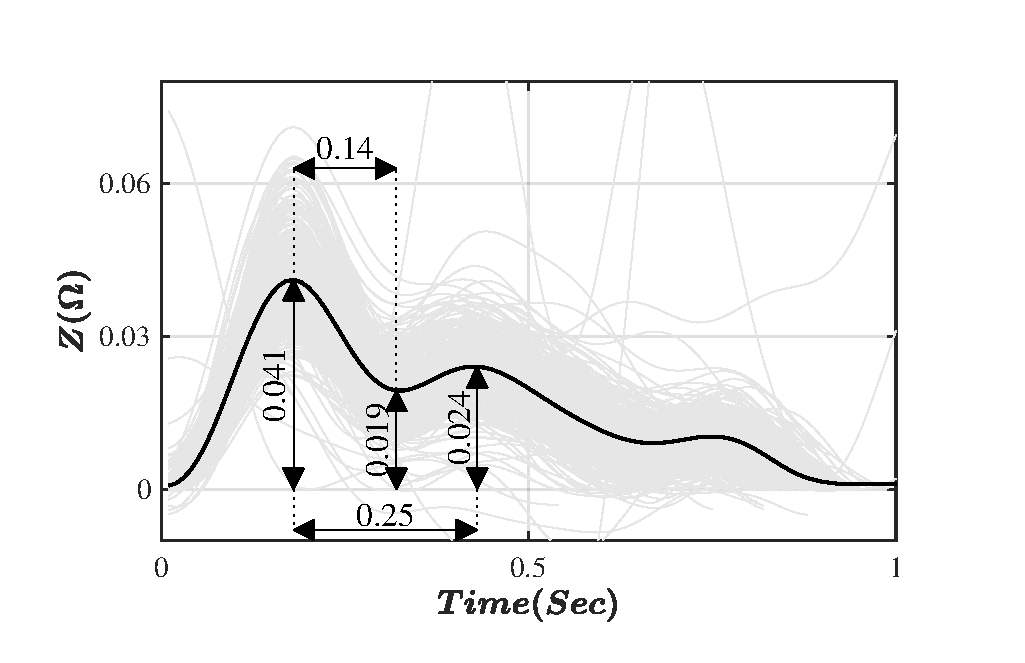
\includegraphics[width=0.45\textwidth, trim={0.5cm 0cm 1.5cm 0 cm}, clip]{figure_apa_6a}}%
	\hfill%
	\subcaptionbox{Average plethysmography waveform during venous occlusion region 6 (\SIrange{1260}{1440}{\second})\label{fig:iPG_total_occlusion}}
	[0.45\textwidth]{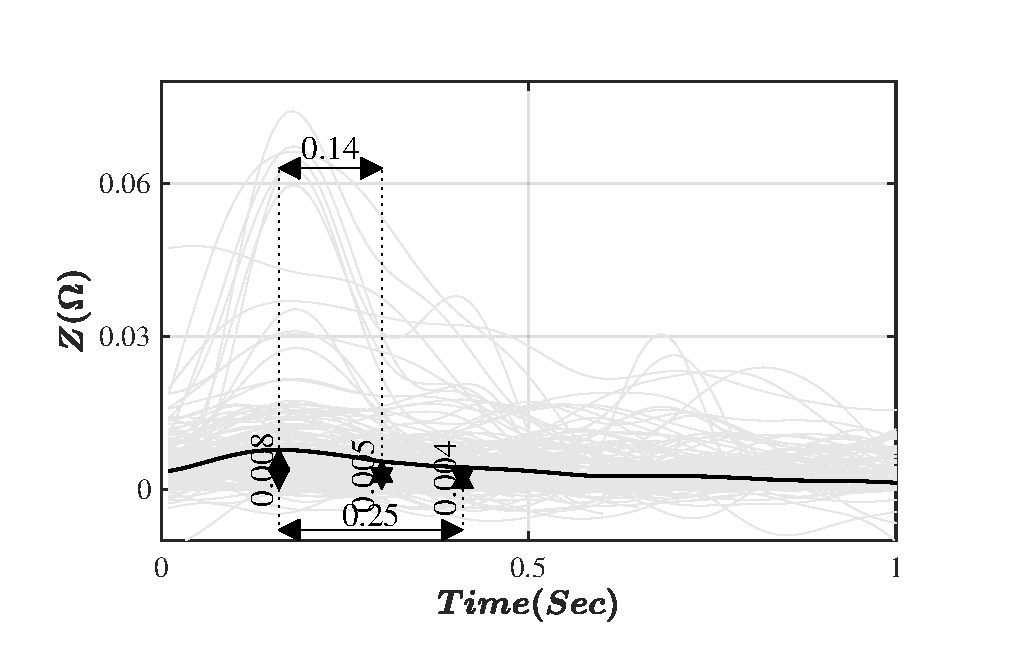
\includegraphics[width=0.45\textwidth, trim={0.5cm 0cm 1.5cm 0 cm}, clip]{figure_apa_6b}}%
	\hfill\null%
	\caption{Plethysmography waveform of the participant seven between baseline and total occlusion}
	\label{fig:iPG_total}
	
	\vspace{1cm}
	
	\null\hfill%
	\subcaptionbox{Change of amplitude of the waveform at point A.\label{fig:change_A_total}}
	[0.48\textwidth]{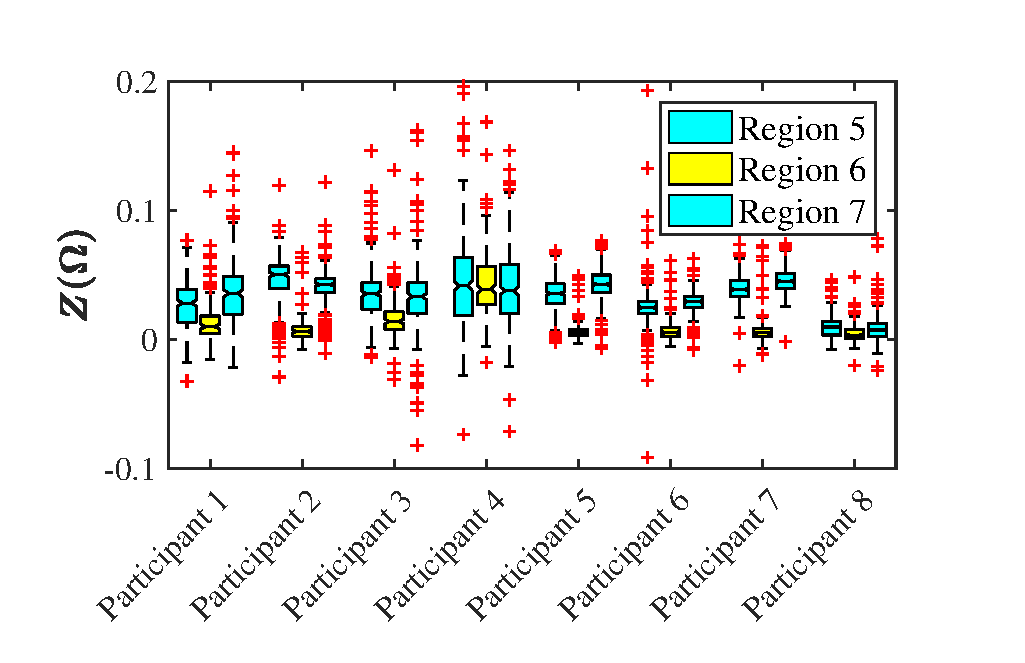
\includegraphics[width=0.45\textwidth, trim={0.5cm 0cm 1.5cm 0 cm}, clip]{figure_apa_7a}}%
	\hfill%
	\subcaptionbox{Change of amplitude of the waveform at point B.\label{fig:change_B_total}}
	[0.48\textwidth]{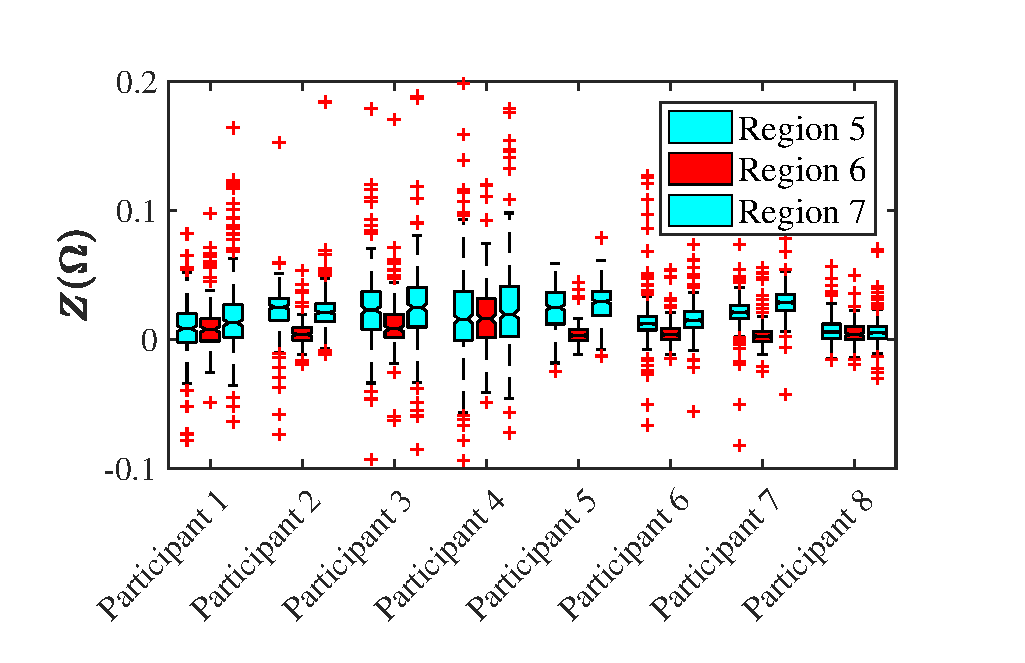
\includegraphics[width=0.45\textwidth, trim={0.5cm 0cm 1.5cm 0 cm}, clip]{figure_apa_7b}}%
	\hfill%
	\subcaptionbox{Change of amplitude of the waveform at point C.\label{fig:change_C_total}}
	[0.48\textwidth]{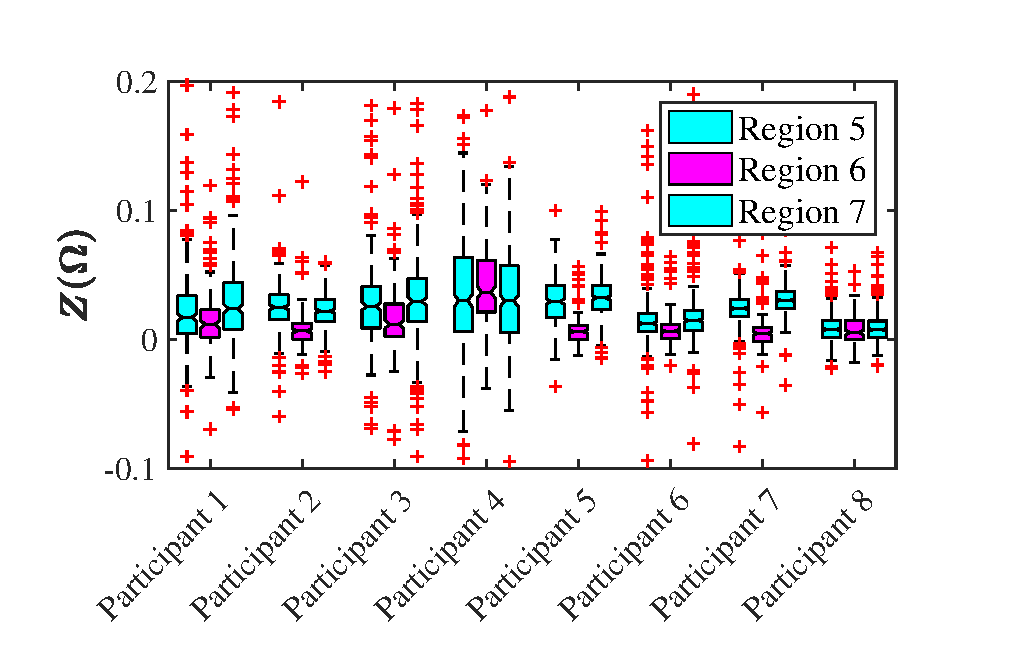
\includegraphics[width=0.45\textwidth, trim={0.5cm 0cm 1.5cm 0 cm}, clip]{figure_apa_7c}}%
	\null%
	\caption{Changes of the impedance peak values during baseline, total occlusion and return to baseline for points A,B and C.}
	\label{fig:iPG_change_points_total}
\end{figure*}

It was observed that performing a total occlusion completely blocks both the inflow and outflow of blood below the arm's cuff.  This implies that there is no change of volume within the arm's segment. As a result, it can be surmised that impedance plethysmography must not present the changes in magnitude.  Figure \ref{fig:iPG_total} shows the APA waveform during the baseline in region 5 (\SIrange{960}{1260}{\second}) and the total occlusion in region 6 (\SIrange{1260}{1440}{\second}) of the seventh participant. As clearly illustrated by the figure \ref{fig:iPG_change_points_total}, the amplitudes of most participants reduced during the occlusion. However, participant 4 experienced different behaviours across all these points. The member's standard deviation also suggests a problem with his plethysmography signal during this test. 

In general, point A decreased by \SI{-66.15}{\percent} on average at its peak value occlusion. Upon the release of pressure, impedance recovered its value in \SI{75.98}{\percent}. A similar event occurred at point B; peak signals reduced by a median of \SI{-63.29}{\percent} during blockage and recovered on average by \SI{74.02}{\percent}. Similarly, point C decreased (on average) by \SI{-50.27}{\percent} and rose by \SI{58.71}{\percent} following the occlusion.

\section{Basal impedance over APA ratio} %Section - 7.2
\label{section discussion 4}

Despite the healthy correlation between DU's amplitude and the iPG's waveform (see chapter \ref{chapter data collection}), their blood flow rates do not provide sufficient details about either venous or arterial occlusions. However, the information provided by the designed iPG devices seems to present further details that might give us a clue about the type of circulatory problem. 

As described before in chapter \ref {chapter basal}, the basal impedance was used to find venous problems by incorporating the venous occlusion technique. However, when an arterial blockage occurs, a similar response is observed, which makes it more difficult to identify the exact location of problem. Meanwhile the amplitude of impedance plethysmography waveform might provide additional details on how to discern between the two kinds of occlusions. Perhaps combining these two data sets would make it possible to discriminate between an appropriate level of circulation as well as an arterial and circulatory problem. 

\begin{figure}[!htpb]
	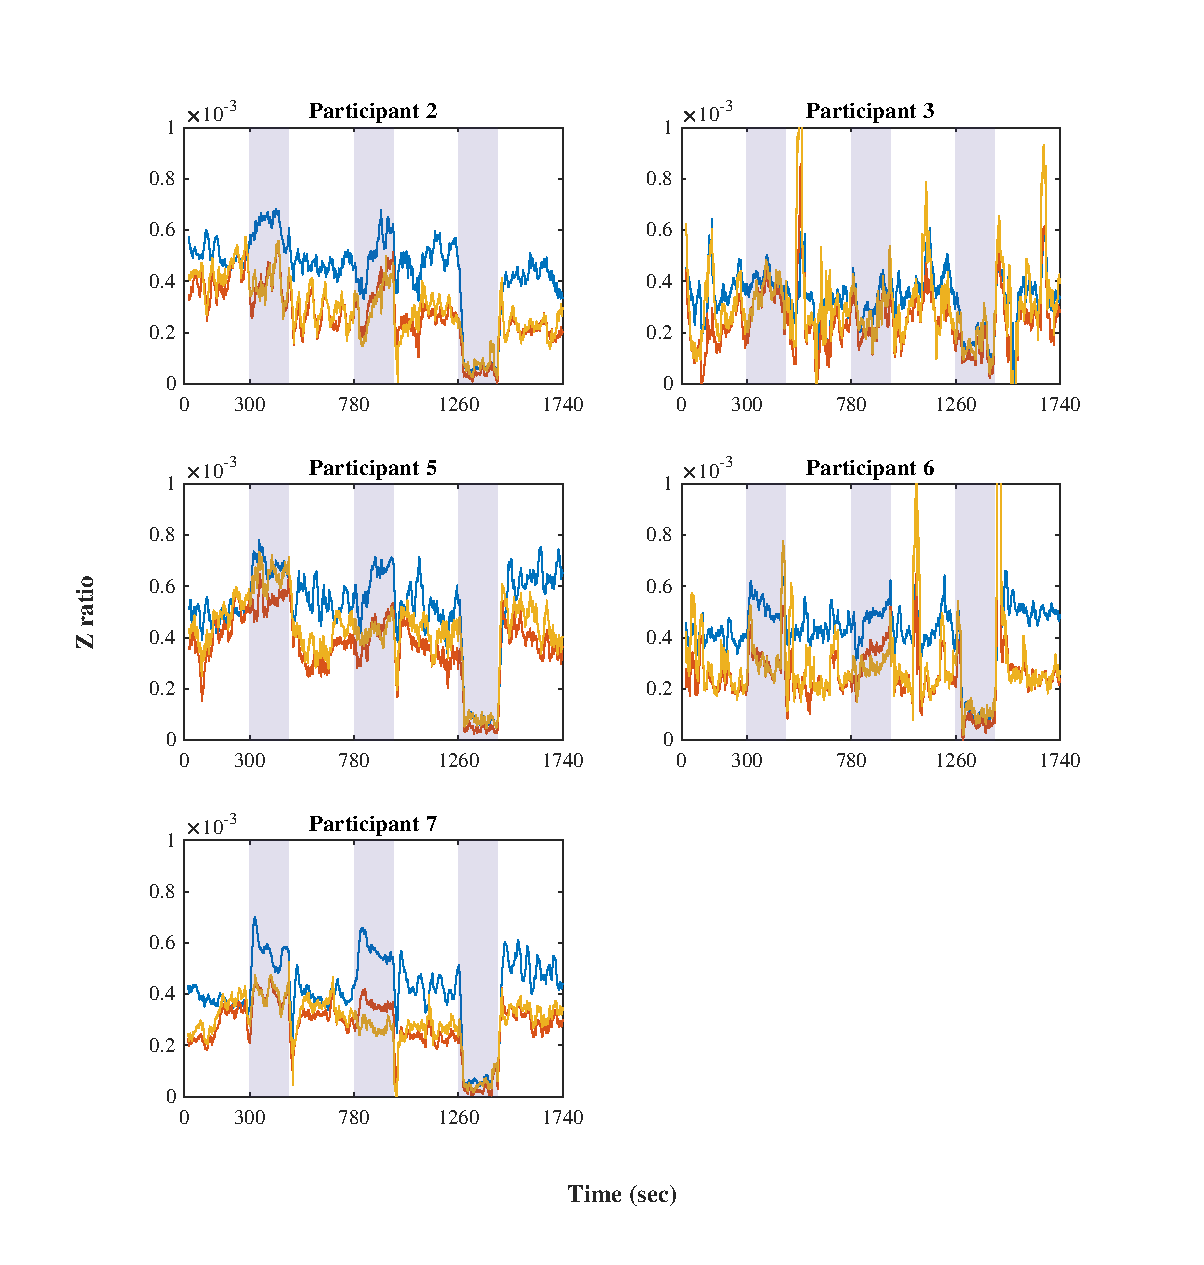
\includegraphics[width=1\textwidth,keepaspectratio]{figure_apa_8}    
	\caption[Ratio of the plethysmography waveform over basal impedance during the experiment]{Measurement of the ratio between the plethysmography waveform over basal impedance during the whole experiment. The blue line represents the systolic peaks (\textit{Point A}), the yellow line the dicrotic notch (\textit{Point B}) and the red line the diastolic peak (\textit{Point C})}
	\label{fig:ratio Z}
\end{figure}

Therefore, a ratio indicator is proposed between the plethysmography waveform and the basal impedance to differentiate between venous and arterial problems. To do so, it is imperative to identify the three points of the plethysmographic waveform: systolic peak, dicrotic notch, and diastolic peak. The ratio can be calculated using the following equation.

\begin{align}
	\label{eq:ratio Z}
	i_Z = \frac{Z_{PG}}{Z_{BAS}}
\end{align}


This is a dimensionless index with three indicators referencing each point of the plethysmography waveform. The method was applied to the study participants, and the results were outlined in figure \ref{fig:ratio Z}. As illustrated by the graph, for most part of the data, the systolic peak is beyond the two other signals. When a venous or partial arterial occlusion occurs (regions 2 and 4), an increment takes place in the index. 

The dicrotic notch and the diastolic peak seem to change as a matching pair for majority of the baseline signals; the dicrotic notch appears to be slightly lower than the diastolic peak. However, at the time of partial arterial blockage, the systolic index reduces below the dicrotic notch index. This event is a clear differentiator between the two types of flow restriction.

\subsection{Evaluation of blood obstructions using iPG DC over AC waveforms}  %Section - 7.3 
\label{section discussion 5}
It can be seen that the estimation of blood from the impedance signal could not be a good enough indicator of circulatory disturbances in either the arterial or venous path. One plausible reason for this could be that the mathematical expression describes a direct relation between the amplitude of the wave and the estimation of blood flow. However, when a mechanical constriction of the arm occurs in either the venous or arterial circulation, there is an increase in amplitude of the waveform. As a result, this increase in the $\Delta R$ will be calculated as a surge in blood flood, which is not an accurate conclusion in entirety. 

Therefore, a method is proposed where it becomes possible to detect problems within the circulatory path by quantifying and analysing the differences within the waveform of the impedance plethysmography signal shape. As described in the section \ref{section apa 1}, three reference points can be used to describe an impedance plethysmography waveform. Typically, a non-disturbed waveform is represented as a systolic peak (point A) that is higher than the diastolic peak (point C) and the dicrotic notch point (point B) lower than those peaks. 

However, when the venous occlusion occurs, it is evident that changes occurring in the waveform shape are distinguishable with each phenomenon. As figure \ref{fig:ration Z bar} reflects, the first noticeable event is that the systolic peak increases in size. This gain in size could be attributed to the blood pooling in the veins. The venous occlusion experienced this effect along with the partial arterial occlusion. However, it must be observed that partial arterial blockage is also a type of venous occlusion wherein it curbs the blood flow towards the forearm. Hence, it is also expected to witness an increase in the systolic peak. 

Additionally, during the venous occlusion, it can be seen that most participants exhibited an increase in the magnitude of dicrotic notch and diastolic peak. Thus, it can be implied that the increase in the impedance plethysmography waveform may signify a restriction of the venous circulation towards the forearm. 

However, this is not the lone indicator of a venous circulatory problem. The basal impedance also tends to vary during this kind of occlusion owing to the increase of blood volume within the veins. Consequently, the basal impedance also decreases over time, which is also an indicator of circulatory problem. Thus, presenting these two values in a single quantifying number could be a more accurate indicator of the restriction in blood flow. 

\begin{figure}[!htpb]
	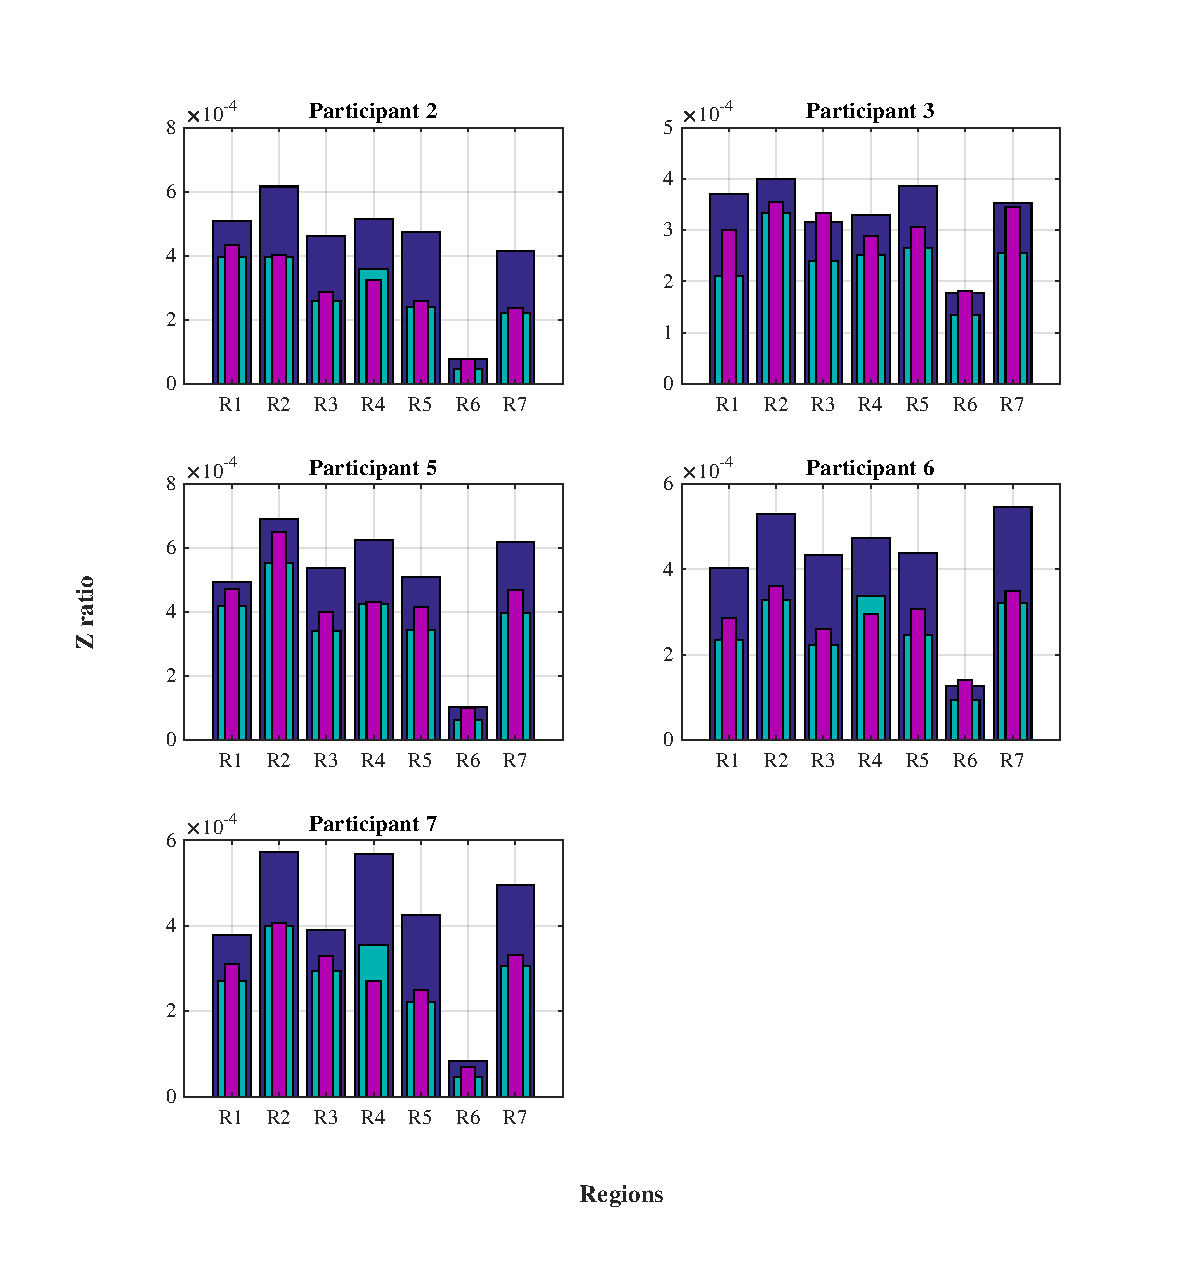
\includegraphics[width=1\textwidth,keepaspectratio]{figure_apa_9}    
	\caption[Bland and Altman plot of the relation between LDF and iPG]{Representation of the index ratio of the APA waveform for each region. The dark purple represents the ratio $\Delta R/ R$ of the systolic peak (point A), the light purple denotes the ratio at the dicrotic notch (point B), and the cyan refers to the magnitude at diastolic peak (point C).}
	\label{fig:ration Z bar}
\end{figure}

\section{Conclusions}
\label{section apa 4}
The iPG signals provided additional information about blood distribution during the occlusive events. The oscillations of the APA signal are attributed to the expansion of arteries and veins during the heart cycle, thereby creating small changes in the impedance. While this tiny waveform is contained within the basal impedance, it is merely a fraction of it. 

The designed impedance device in its entirety, including hardware and software algorithms, was able to identify the plethysmography waveforms by localising distinctive landmarks such as the systolic peak, dicrotic notch and diastolic point. Obtaining this level of detail was vital because it provided more details about the changes occurring in different segments of the impedance plethysmography waveform. From this premise, it could recognise the changes in shape during each types of occlusions performed during the test.  It is evident that at the time of each occlusive event, the amplitude of systolic and diastolic peaks manifested a particular response in accordance to the type of blood flow restriction. Notably, the waveform shape might be unique to this kind of set-up, and it is possible that altering the electrodes distance or using different frequencies may impact the impedance waveform.

Meanwhile changes were observed in the size of the systolic peak (point A), dicrotic notch valley (point B) and diastolic peak (point C) when an occlusion took place. The increase in size might be attributed to a physiological response during the occlusion where the volume capacity of veins increased to accommodate the pooled blood. An example of this is evident in figure \ref{fig:iPG change points venous} which described the differences between region 1, 2 and 3. According to the figure, there was an increase in the size of all reference points in majority of the participants during the occlusion, which was followed by a return to the baseline. However, the observations made in the partial occlusion for regions 3, 4 and 5 suggested that while the systolic peak did increase in size, the dicrotic notch and diastolic peak declined in amplitude when compared to the venous occlusion and baseline waveform. The difference in waveform is an accurate indicator of an obstruction in either a arterial or venous circulation. 

The chapter \ref{chapter basal} demonstrated that during the occlusions, a different slope was noted during in each kind of occlusion. By combining the information of basal impedance with the APA waveform, it is possible to generate a 3-point ratio index that could be indicative of a potential obstruction within the forearm. This observation suggested that if there is a significant increase in the relation index of the systolic peak, it could be the first prominent indicator of circulatory blockage. On the other hand, an increase in the dicrotic notch and the diastolic peak indicates that the occlusion might occur in the venous return if the dicrotic notch ratio index is higher than the other following one. While undertaking a comparison, the data showed that if there is a surge in systolic peak size, the dicrotic notch amplitude tends to reduce or is at similar amplitude of the diastolic point; it might then be an indicator of an imminent arterial occlusion.




%********************************** %Nomenclature found  *************************************

